\documentclass{beamer}
\usepackage{listings}
\usetheme{Copenhagen}
\usecolortheme{beaver}
\setbeamertemplate{navigation symbols}{}
\setbeamertemplate{footline}{\parbox[t][12pt][c]{12pt}{~\scriptsize\insertframenumber}}
% \usepackage{beamerthemesplit} // Activate for custom appearance

%%%%%%%%%%%%
% MVS: Language definitions
%
\renewcommand{\ttdefault}{pcr}
\lstset{
  basicstyle=\small\ttfamily,
  breaklines=true
}
\lstdefinelanguage{cvl}{
  morekeywords={generalize,to, with, other, at, zoom, levels, weigh, by, subject, and, create, constraint, as, not, exists, resolve, if, delete, select, from, where, in, order, over, setup, teardown,force,min,level,for,allornothing,join,on,setup,group,having,index,temporary,table,drop,partition,merge,partitions},
  sensitive=false,
  morecomment=[l]{//},
  morecomment=[s]{/*}{*/},
  morestring=[b]",
}
\lstset{
  language=cvl
}


\title{Declarative Cartography}
\subtitle{In-Database Map Generalization of Spatial Datasets}
\author{\underline{Pimin Konstantin Kefaloukos}, Marcos Vaz Salles, \\Martin Zachariasen\\ \small{\emph{Computer Science Department (DIKU)}, \textbf{University of Copenhagen}}}

\date{\today}

\begin{document}

\frame{\titlepage}

\frame
{
  \frametitle{Motivation}
  \begin{itemize}
  \item \textbf{Imagine}: you're a \emph{data journalist} and want to tell a story about restaurants in Z\"{u}rich \emph{using a map}.
  \item \textbf{Database}: You have a \emph{database} of restaurants (unique ID, location, star rating, name etc.)
  \item Simply showing all the records creates a mess (see picture)
  \item Generalization of thematic data is an important problem, with increasing use cases in \emph{social networks}, \emph{data journalism} etc
  \end{itemize}
  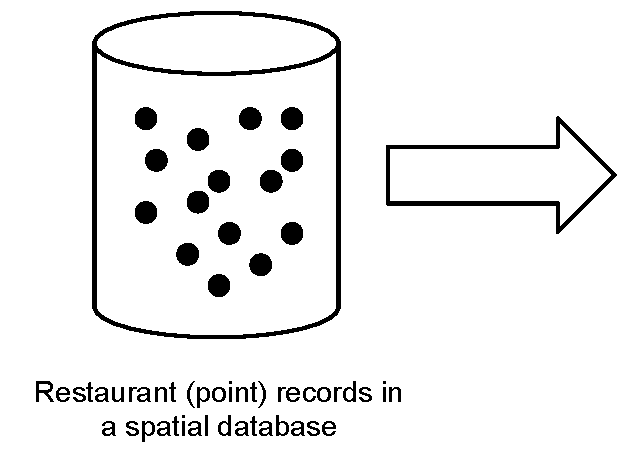
\includegraphics[scale=0.5]{figs/spatial-database-with-points.pdf} 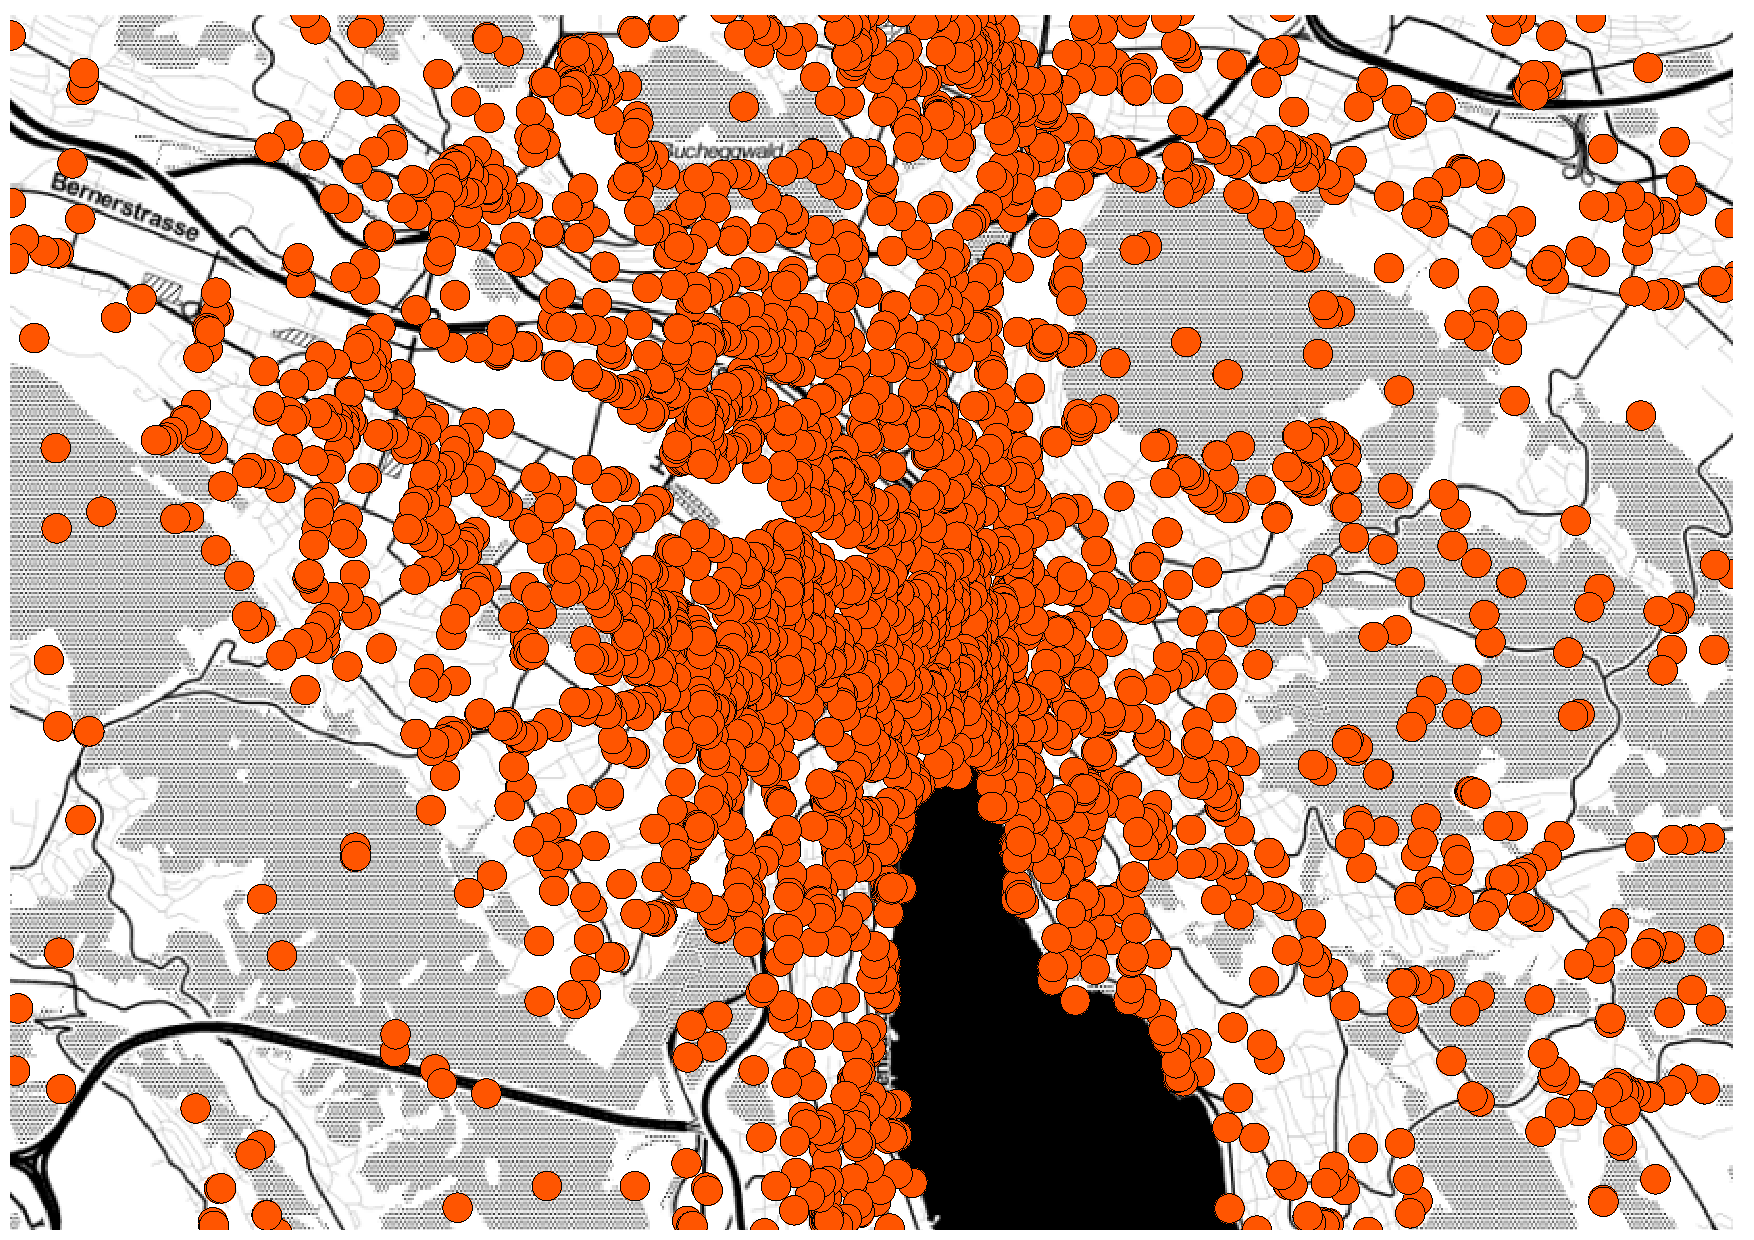
\includegraphics[scale=0.18]{figs/zurich-unfiltered.pdf}
}

% Setting stage
\frame[t]
{
  \frametitle{What a good (thematic) map might look like}
\begin{columns}[t]
	\begin{column}[l]{6cm}
		\begin{itemize}[<+->]
			\item Records should appear \emph{gradually} when zooming in, i.e. \emph{constant information~density}
			\item ``Important'' records should get priority
			\item Visible records should \emph{remain visible} when zooming in
			\item There should be some way of imposing \emph{constraints}
		\end{itemize}
	\end{column}
	\begin{column}[l]{6cm}
    \begin{figure}
    	\includegraphics<1>[scale=0.18]{figs/zoom12.pdf}
        \includegraphics<2>[scale=0.18]{figs/zoom13.pdf}
        \includegraphics<3>[scale=0.18]{figs/zoom14.pdf}
        \includegraphics<4>[scale=0.18]{figs/zoom15.pdf}
    \end{figure}                            
\end{column}
\end{columns}
}


% Setting stage
\frame[t]
{
  \frametitle{Spatial databases}
	\begin{itemize}[<+->]
		\item Spatial data is often stored in a \emph{spatial database}
		\item Databases have powerful capabilities
		\item \emph{joins}, \emph{sorting}, \emph{spatial indexing} and \emph{spatial functions}
	\end{itemize}
	\begin{center}
	\begin{figure}
    		\includegraphics<1>[scale=0.3]{figs/cvl-powerful-database.pdf}
    		\includegraphics<2>[scale=0.3]{figs/cvl-powerful-database.pdf}
		\includegraphics<3>[scale=0.3]{figs/cvl-powerful-database-2.pdf}
	\end{figure}       
	\end{center}                     
}

\frame[t]
{
  \frametitle{Situation}
	\begin{itemize}[<+->]
		\item Normally data is \emph{pulled out} of the database for processing tasks like generalization
		\item Generalization algorithms are usually implemented in external software
		\item After the processing is done the data is put back into the database
		\item \emph{Several drawbacks}: re-inventing the wheel, memory and bandwidth limits, development and deployment costs, 
	\end{itemize}
	\begin{center}
	\begin{figure}
    		\includegraphics<1>[scale=0.3]{figs/cvl-external-software-out.pdf}
    		\includegraphics<2>[scale=0.3]{figs/cvl-external-software-proc.pdf}
		\includegraphics<3>[scale=0.3]{figs/cvl-external-software-in.pdf}
		\includegraphics<4>[scale=0.3]{figs/cvl-external-software-rest.pdf}
	\end{figure}       
	\end{center}                     
}

\frame[t]
{
  \frametitle{Why not use the database itself?}
	\begin{itemize}[<+->]
		\item Instead, we will state generalization in terms of a high-level programming language
		\item High-level programs are translated (compiled) to low-level database programs
		\item We move code-to-data instead of moving data-to-code

	\end{itemize}
	\begin{center}
	\begin{figure}
    		\includegraphics<1>[scale=0.3]{figs/cvl-state-intension.pdf}
    		\includegraphics<2>[scale=0.3]{figs/cvl-compile-statement.pdf}
		\includegraphics<3>[scale=0.3]{figs/cvl-code-to-data.pdf}
	\end{figure}       
	\end{center}                     
}


\frame[t]
{
  \frametitle{In-database processing}
	\begin{itemize}[<+->]
		\item The low-level program can of course exploit capabilities of spatial databases, such as indexing and spatial functions
		\item What exactly do we mean by generalization?
	\end{itemize}
	\begin{center}
	\begin{figure}
    		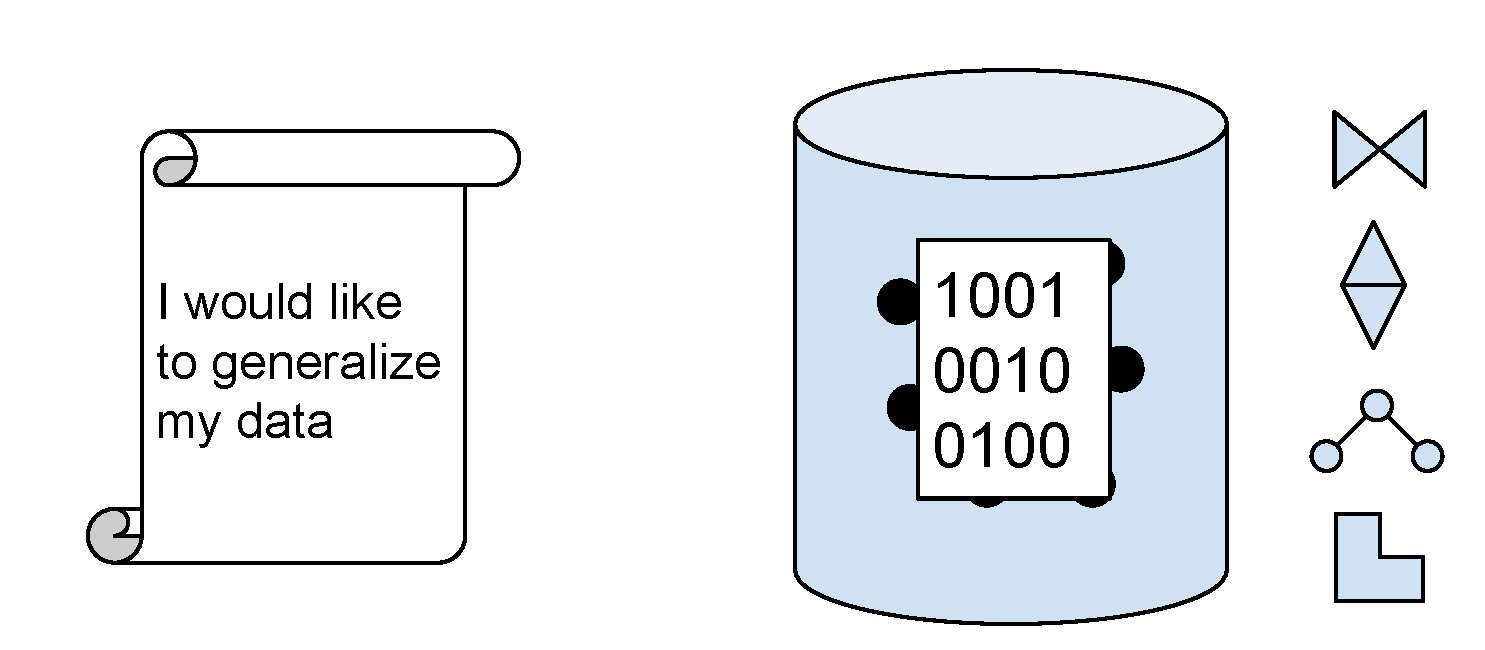
\includegraphics[scale=0.4]{figs/cvl-code-to-data-exploit.pdf}
	\end{figure}       
	\end{center}                     
}

\frame[t]
{
  \frametitle{What we mean by generalization}
	\begin{itemize}[<+->]
		\item \textbf{Input}: table with \texttt{ID}, \texttt{Geometry} and additional columns
		\item \textbf{Output}: input table extended with \texttt{MinZoom} column
		\item Value of \texttt{MinZoom} is the zoom level $z \in \lbrack 1, \mathcal{Z} \rbrack$ when a record becomes visible in the map
		\item Any assignment of \texttt{MinZoom} corresponds to a particular generalization of the data
		\item $O(\mathcal{Z}^n)$ many ways to assign a value to \texttt{MinZoom} for $n$ records
	\end{itemize}
	\vspace{1em}
	\begin{columns}[t]
		\begin{column}[l]{4cm}
  		\includegraphics<1>[scale=0.35]{figs/cvl-table-before-after.pdf}
		\includegraphics<2>[scale=0.35]{figs/cvl-table-before-after-2.pdf}
		\includegraphics<3>[scale=0.35]{figs/cvl-table-before-after-2.pdf}
		\includegraphics<4>[scale=0.35]{figs/cvl-table-before-after-2.pdf}
		\includegraphics<5>[scale=0.35]{figs/cvl-table-before-after-2.pdf}
		\end{column}
		\begin{column}[r]{4cm}
		\includegraphics<3>[scale=0.30]{figs/cvl-problem.pdf}
		\includegraphics<4>[scale=0.30]{figs/cvl-problem.pdf}
		\includegraphics<5>[scale=0.30]{figs/cvl-problem.pdf}
		\end{column} 
  	\end{columns}
}

\frame[t]
{
  \frametitle{Guiding the generalization}
  \begin{itemize}[<+->]
  \item All records in table are assigned a \emph{weight} representing their ``importance''
  \item Visible records must satisfy \emph{spatial constraints}
  \item Objective is to \emph{minimize} the combined weight of non-visible records (records filtered out to satisfy constraint)
  \vspace{1em}
  \end{itemize}
  	\begin{columns}[t]
		\begin{column}[l]{4cm}
  		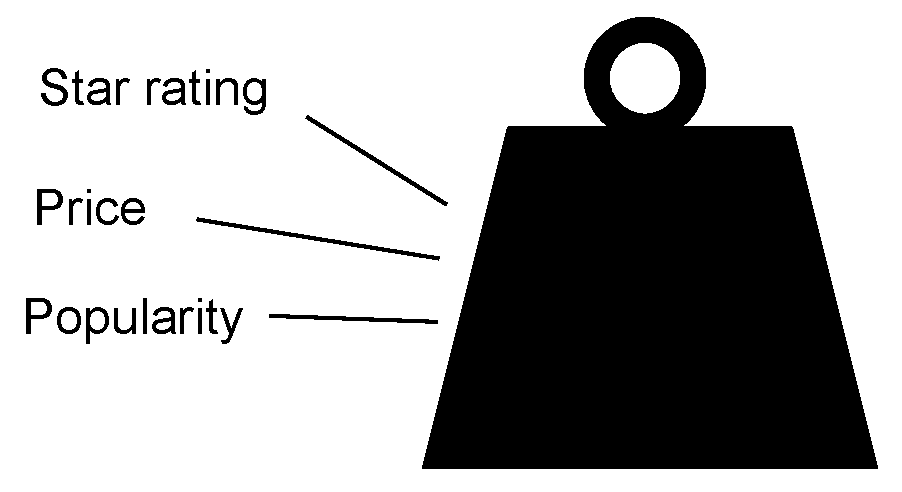
\includegraphics[scale=0.27]{figs/cvl-weight.pdf}
		\end{column}
		\begin{column}[r]{4cm}
		\includegraphics<3>[scale=0.30]{figs/cvl-proximity.pdf}
		\end{column} 
  	\end{columns}

}

\frame{
	\frametitle{Expressing generalization in a programming language}
	\begin{itemize}[<+->]
	\item How to formulate the task of generalizing data in the high and low-level languages?
	\end{itemize}
}

% Introduce syntax
\begin{frame}[fragile,t]
  \frametitle{High-level language example}
  \begin{description}[<+->]
  \item
  \begin{lstlisting}
GENERALIZE restaurants 
\end{lstlisting}
  \item
\begin{lstlisting}
TO restaurants2
\end{lstlisting}
  \item
\begin{lstlisting}
AT 20 ZOOM LEVELS
\end{lstlisting}
  \item
\begin{lstlisting}
WEIGH BY star_rating
\end{lstlisting}
  \item
\begin{lstlisting}    
SUBJECT TO proximity 10 AND density 64
\end{lstlisting}
  \item
    \begin{center}
  	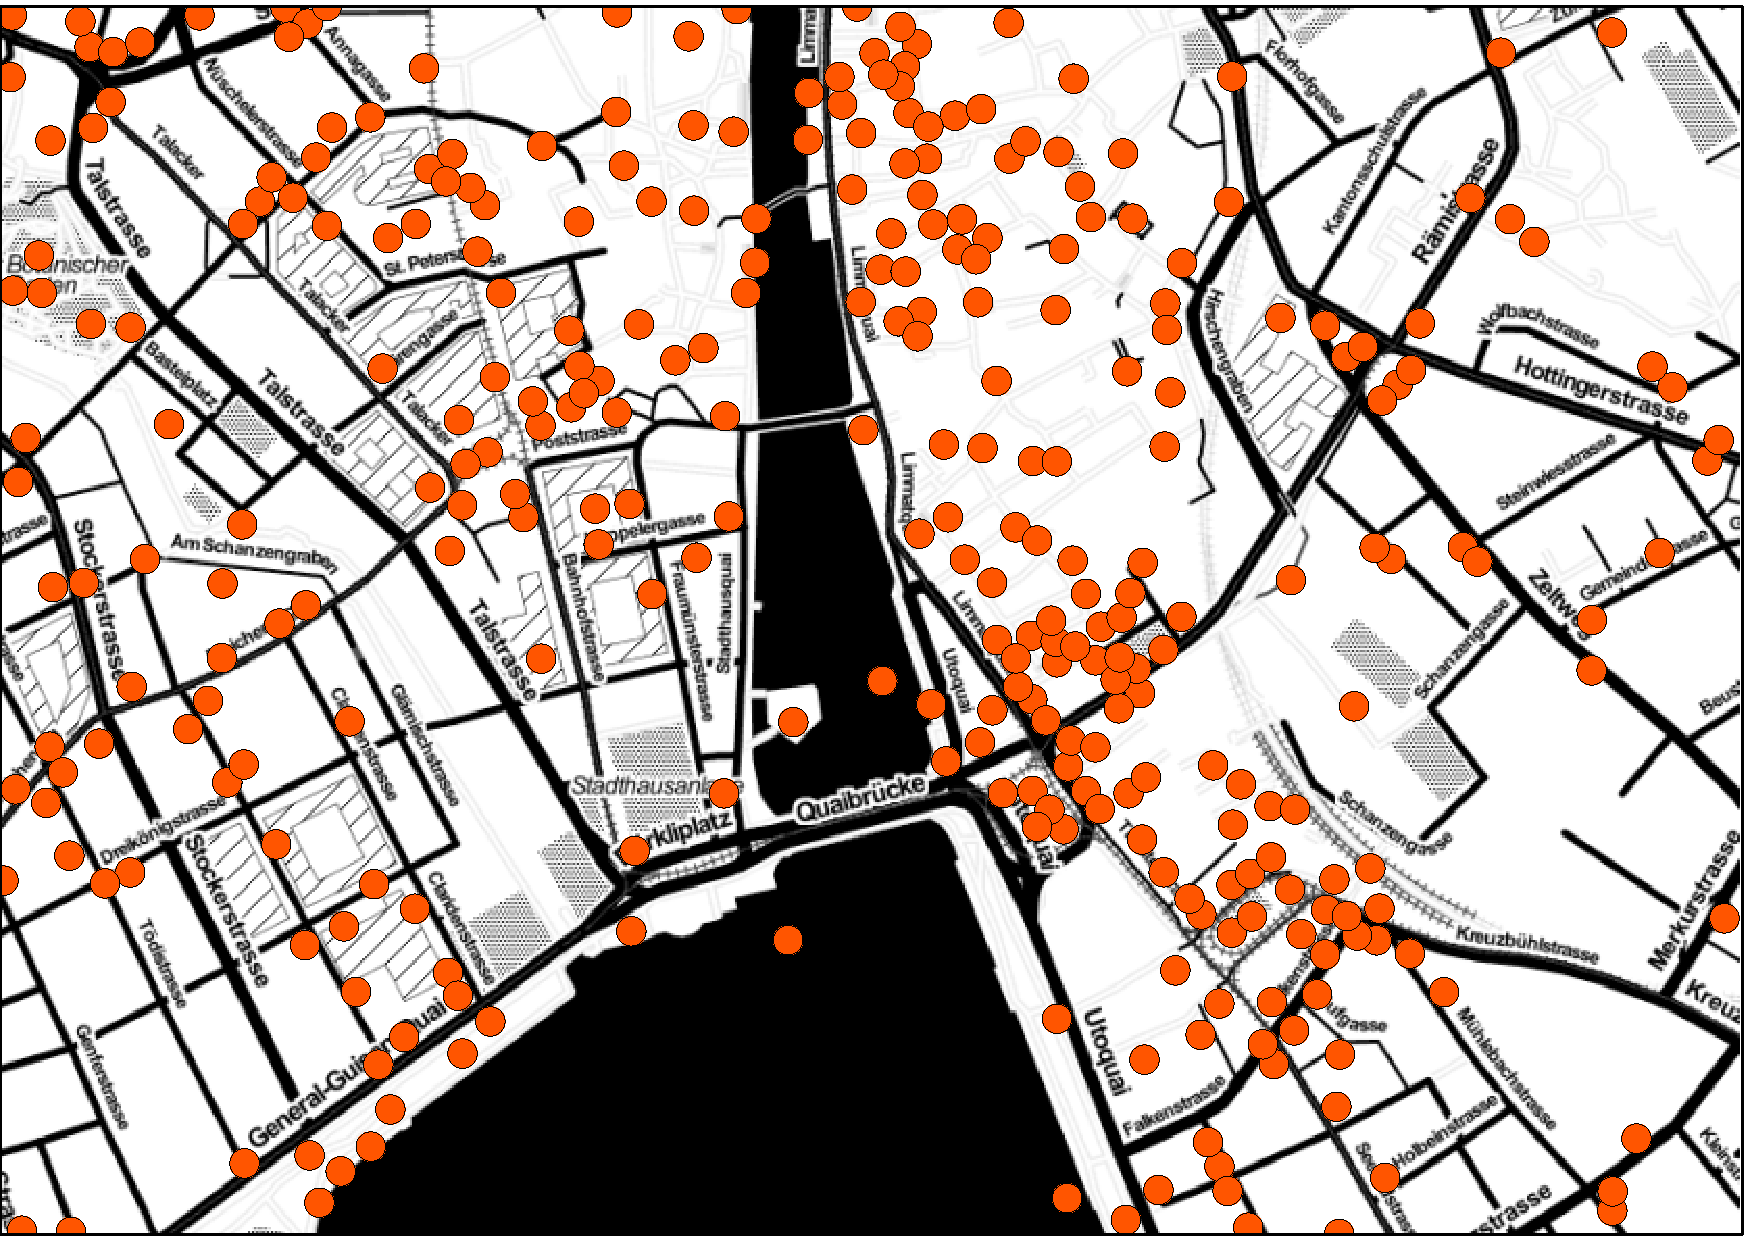
\includegraphics[scale=0.15]{figs/zoom16.pdf}
  \end{center}
  \end{description}
\end{frame}

\begin{frame}[fragile]
\frametitle{CREATE CONSTRAINT statement}
\begin{lstlisting}
CREATE CONSTRAINT {name}
AS NOT EXISTS
  {SQL select statement}
  
RESOLVE cid IF DELETE (
  {integer expression}
)
\end{lstlisting}
\end{frame}

\begin{frame}[fragile]
\frametitle{Example usage}
\begin{lstlisting}
CREATE CONSTRAINT Proximity
AS NOT EXISTS (
  SELECT l.id || r.id AS cid, 
    Unnest(array[l.id, r.id]) AS rid
  FROM
    {level_view} l JOIN {level_view} r
  ON
    l.id < r.id
  AND
    l.geom && ST_Expand(r.geom, 
      CVL_Resolution({z}, 256) * {parameter_1})
  AND
    ST_Distance(l.geom, r.geom) < 
      CVL_Resolution({z}, 256) * {parameter_1}
)

RESOLVE cid IF DELETE (
  1
)
\end{lstlisting}
\end{frame}

\frame[t]
{
  \frametitle{Computing solutions}
	\begin{itemize}[<+->]
	\item Combination of record weights and spatial constraints (proximity, density) present a natural optimization problem
	\item Mapping to set multicover problem (SMP)
	\item Reuse existing algorithms for SMP (database implementations)
	\end{itemize}
	\begin{center}
  		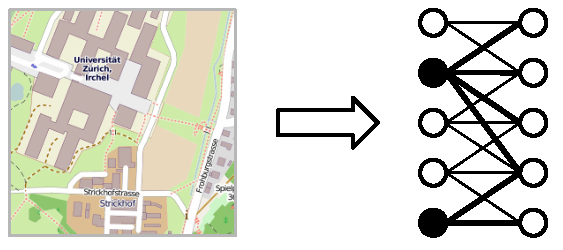
\includegraphics[scale=0.70]{figs/cvl-spatial-to-nonspatial.pdf}
  	\end{center}
}

\frame[t]
{
  \frametitle{Computing solutions}
	\begin{itemize}[<+->]
	\item Use auto-generated SQL queries to find records that violate constraints, i.e. find conflict sets
	\item Resolve conflicts by filtering out some records
	\item Minimize combined weight of records that are filtered out over all zoom levels
	\end{itemize}
	
	\begin{center}
	\begin{figure}
  		\fbox{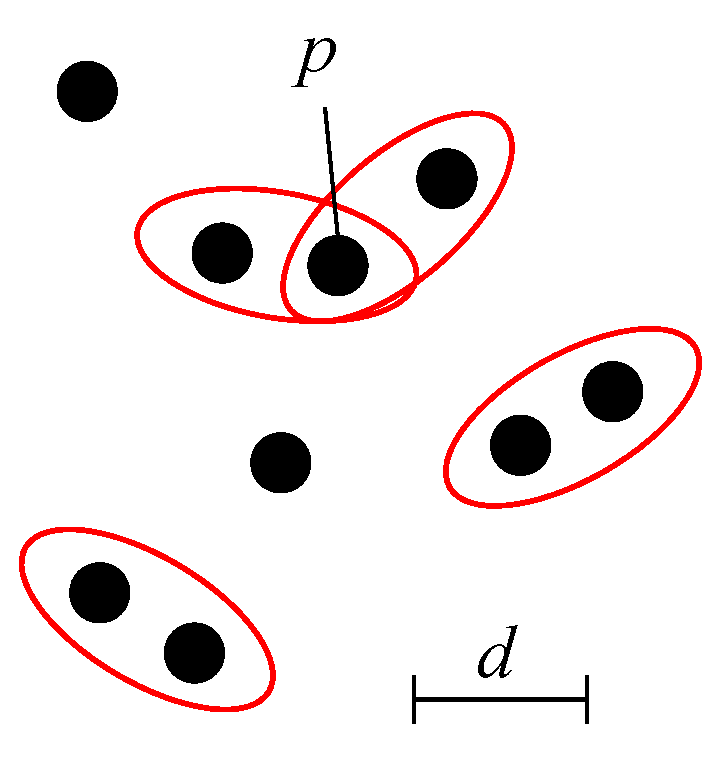
\includegraphics[scale=0.25]{figs/cvl-proximity-conflicts.pdf}}
	\caption{Four conflict sets generated by a proximity constraint}
	\end{figure}
  	\end{center}
}


\frame[t]
{
  \frametitle{Summary}
	\begin{itemize}
	\item Designed a high-level language for generalization called CVL
	\item Compiled to low-level database program and moved code-to-data
	\item Exploited correspondence to well-known optimization problem
	\item Also, method works with both points, lines and polygons
	\end{itemize}
	\begin{center}
	\begin{figure}
  		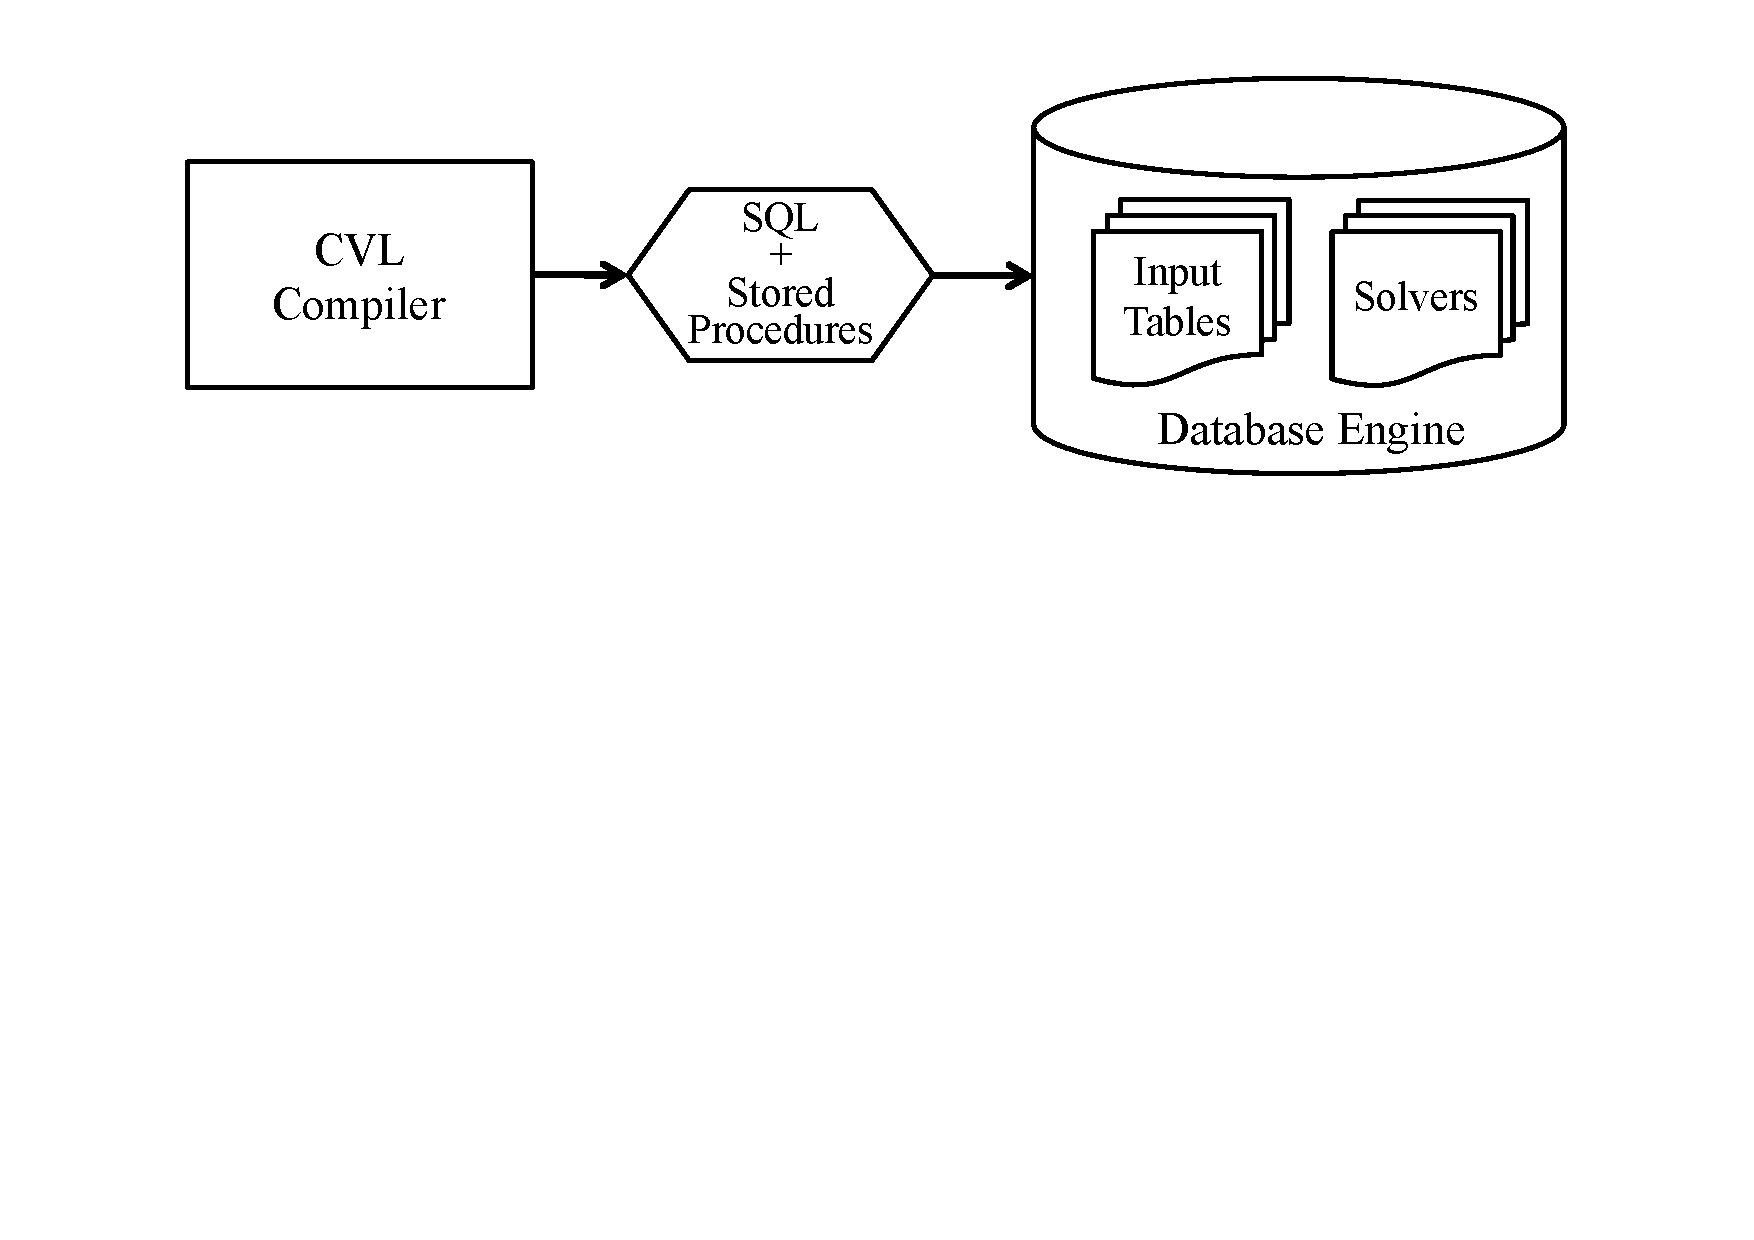
\includegraphics[scale=0.25]{figs/indatabase-execution.pdf}
	\caption{Architecture of CVL}
	\end{figure}
  	\end{center}
}

\frame[t]
{
  \frametitle{Future work}
	\begin{itemize}
	\item Implement aggregation as conflict resolution method
	\item Reduce dependencies of database program code
	\item Optimize low-level code generation
	\item Validate method in comprehensive user tests
	\item Identify areas where method can be further developed
	\end{itemize}
	\begin{center}
	\begin{figure}
  		\fbox{Thank you!}
	\end{figure}
	\end{center}
	\begin{center}
	  	Work will appear at ICDE '14 in Chicago, IL
	\end{center}	
}


\end{document}